%! Author = ruochongli
%! Date = 2023/3/12

% Preamble
\documentclass[./main.tex]{subfiles}

% Packages

% Document
\begin{document}
    \section{Sensitivity Analysis}
    \subsection{Impact from the Population}
    In October 2022, it was announced that a semiconductor fabrication facility $50$ kilometers east of the property
    will be built.
    It will directly and indirectly create about $49,000$ jobs.
    Assume $30\%$ of the workers will move to the city and their families will come with them, then there will be
    about $44,
    000$ additional people living in the city of Clay.

    The fab is closer to the urban center, and shall have more jobs created, so that fewer people will rely on the
    jobs created by our unplanned property in Red Creek.
    Meanwhile, more people will live in urban areas, so it will be important for them to relax in the country, thus
    companies will be more profitable if they develop tourism.
    So we can reduce the weight for employment and raise the weight for population and visitors flow-rate to get a
    more suitable solution.

    Following the solution in Figure~\ref{fg1}, we get Figure~\ref{fig:figurePP}.
    It shows the coefficient of profit changes with the addition in weight for population and
    visitors flow-rate, as well as the subtraction in weight for employment.
    %todo

    \lq\lq{Control}\rq\rq\ in the figure means the control group, which means it was the same as the original coefficient of profit in Figure~\ref{fb1}.
    As the independent variable of the $x$-axis increases, the weight for population, visitors flow-rate and the
    subtraction in weight for employment

    \begin{figure}[H]
        \centering
        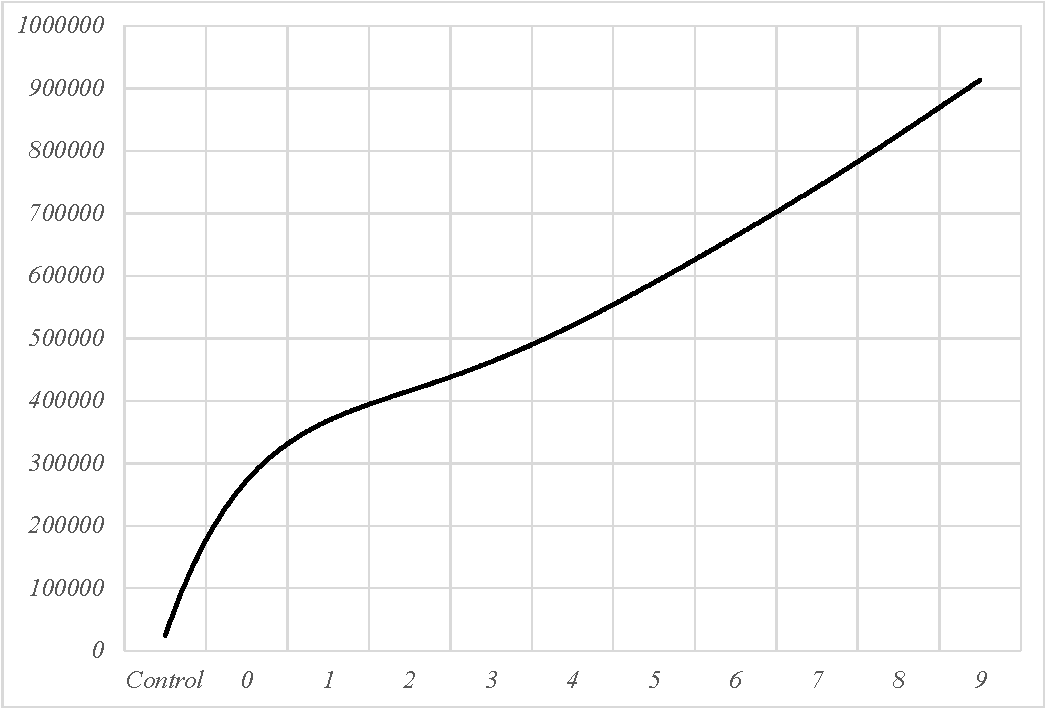
\includegraphics[width=0.75\textwidth]{./figure/figurePP}
        \caption{Impact from the population change}
        \label{fig:figurePP}
    \end{figure}

    With the change, we can see obvious increase in coefficient of profit: increasing from $200,000$ pts to just
    under $1,000,000$ pts.
    Therefore, the population does have a large impact on the solution.
    

    \subsection{Impact from the Number of Metrics}
    With fewer metrics, the coefficient of profit will be more sensitive to any change of the solution and have fewer
    points.
    While making small changes to the overall solution, we decrease the number of metrics that are taken into consider and
    get the result in Figure~\ref{fig:figurePI}

    \begin{figure}[H]
        \centering
        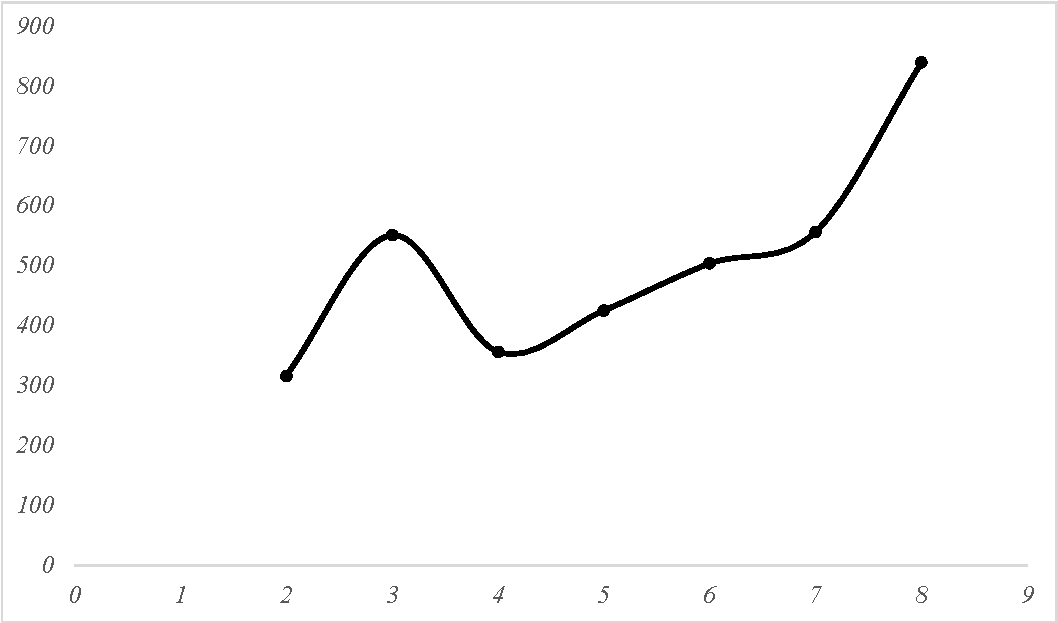
\includegraphics[width=0.75\textwidth]{./figure/figurePI3}
        \caption{Impact from number of metrics}
        \label{fig:figurePI}
    \end{figure}

    From Figure~\ref{fig:figurePI}, we can see a sudden rise at the three metric place, which is in line with our
    prediction.
    
    \subsection{Impact from the Total Time}
    Accounting prime costs, the longer the total time, the more profitable it would get.
    Thus, short-term and long-term benefits or costs should vary significantly.
    We simulate the total time from one year to ten years, with a step size of one year.

    \begin{figure}[H]
        \centering
        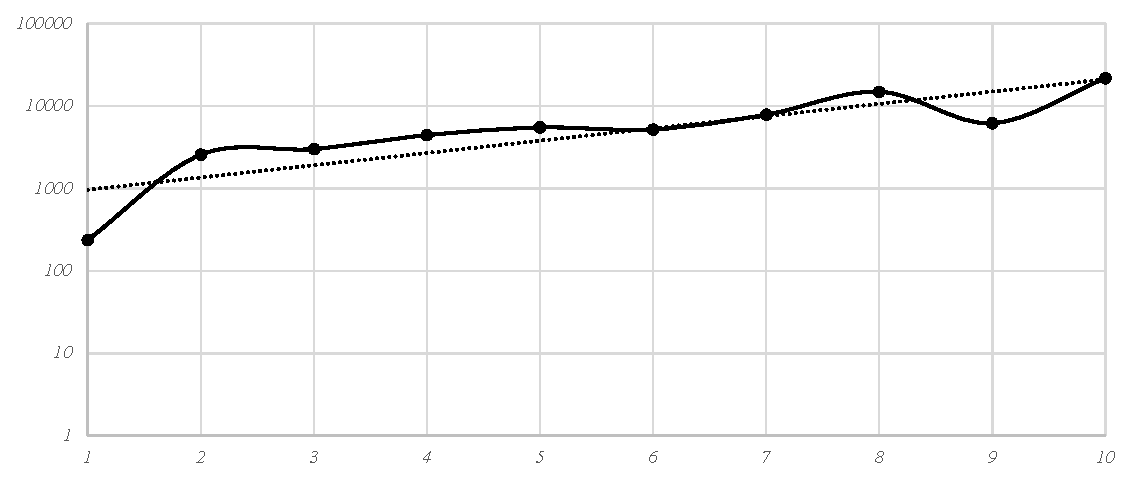
\includegraphics[width=\textwidth]{./figure/figurePT}
        \caption{Impact from Operation Time (log-based $y$-axe)}
        \label{fig:figurePT}
    \end{figure}

    Shown in Figure~\ref{fig:figurePT}, the total time has a linear relationship with the logarithm of coefficient of profit $P$,
    with a goodness of fit of $R^2=0.782$.
    It shows that out model has a reasonably good sensitivity.

\end{document}